\section{Merge Sort}

\subsection{Definition}
\begin{itemize}
    \item Sortieralgorithmus basierend auf Divide-and-Conquer
    \item Wie bei Heap-Sort:
    \begin{itemize}
        \item Benutzung eines Comparators
    \end{itemize}
    \item Anders als beim Heap-Sort:
    \begin{itemize}
        \item keine Benutzung einer Priority-Queue
        \item Zugriff auf Daten sequentiell (geeignet zum Sortieren von Daten auf der Disk)
    \end{itemize}
\end{itemize}

\subsubsection{Divide-and-Conquer (Teile- und-Herrsche)}
Ein generelles Paradigma beim Design von Algorithmen:
\begin{itemize}
    \item \textbf{Divide:} Input-Daten S in zwei getrennte Teilmengen S1 und S2 aufteilen
    \item \textbf{Recur (Wiederhole):} die Teilprobleme mit S1 and S2 rekursiv lösen
    \item \textbf{Conquer:} mischen der Lösungen von S1 und S2 in die Lösung von S
\end{itemize}

\subsection{Laufzeit}
\begin{itemize}
    \item Die Höhe h des Merge-Sort Baumes ist O(log n)
    \item Der Gesamt-Aufwand aller Knoten einer Tiefe i ist O(n)
    \item totale Laufzeit des Merge-Sort ist O(n * log(n))
\end{itemize}


\subsection{Algorithmus}
\begin{itemize}
    \item Input-Sequenz S
    \item n Elementen
    \item 3 Schritte:
    \begin{itemize}
        \item \textbf{Divide:} S in zwei Sequenzen S1 und S2 von je n/2 Elemente aufteilen
        \item \textbf{Recur:} rekursiv S1 und S2 sortieren
        \item \textbf{Conquer:} S1 und S2 in eine sortierte Sequenz mischen
    \end{itemize}
\end{itemize}
\begin{lstlisting}
Algorithm mergeSort(S, C)
    Input sequence S with n elements, comparator C
    Output sequence S sorted according to C
    if S.size() > 1
        (S1, S2) <- partition(S, n/2)
        S1 <- mergeSort(S1, C)
        S2 <- mergeSort(S2, C)
        S <- merge(S1, S2)
    return S
\end{lstlisting}
Mischen von zwei sortierten Sequenzen A und B in die sortierte Sequenz S, enthaltend die Vereinigung der Elemente von A und B\\
Mischen zweier sortierter Sequenzen von je n/2 Elemente mit double-linked Listen: O(n) Laufzeit \\
\subsection{Mischen zweier sortierter Sequenzen}

\begin{lstlisting}
Algorithm merge(A, B)
    Input sequences A and B with n/2 elements each
    Output sorted sequence of A £$\bigcup$£  B

    S <- empty sequence
    while !A.isEmpty() && !B.isEmpty()
        if A.first().element() < B.first().element()
            S.insertLast(A.remove(A.first()))
        else
            S.insertLast(B.remove(B.first()))
    while !A.isEmpty()
        S.insertLast(A.remove(A.first()))
    while !B.isEmpty()
        S.insertLast(B.remove(B.first()))
    return S
\end{lstlisting}

\subsection{Merge-Sort Baum}
\begin{itemize}
    \item Die Ausführung eines Merge-Sort kann als binärer Baum dargestellt werden
    \item Jeder Knoten representiert einen rekursiven Aufruf des Merge- Sort und enthält:
    \begin{itemize}
        \item unsortierte Sequenz vor der Ausführung und der Aufteilung
        \item sortierte Sequenz nach dem Ende der Ausführung
    \end{itemize}
    \item Wurzel entspricht dem initialen Aufruf
    \item Blätter sind Aufrufe auf Teilsequenzen der Grösse 0 oder 1
\end{itemize}
\begin{center}
    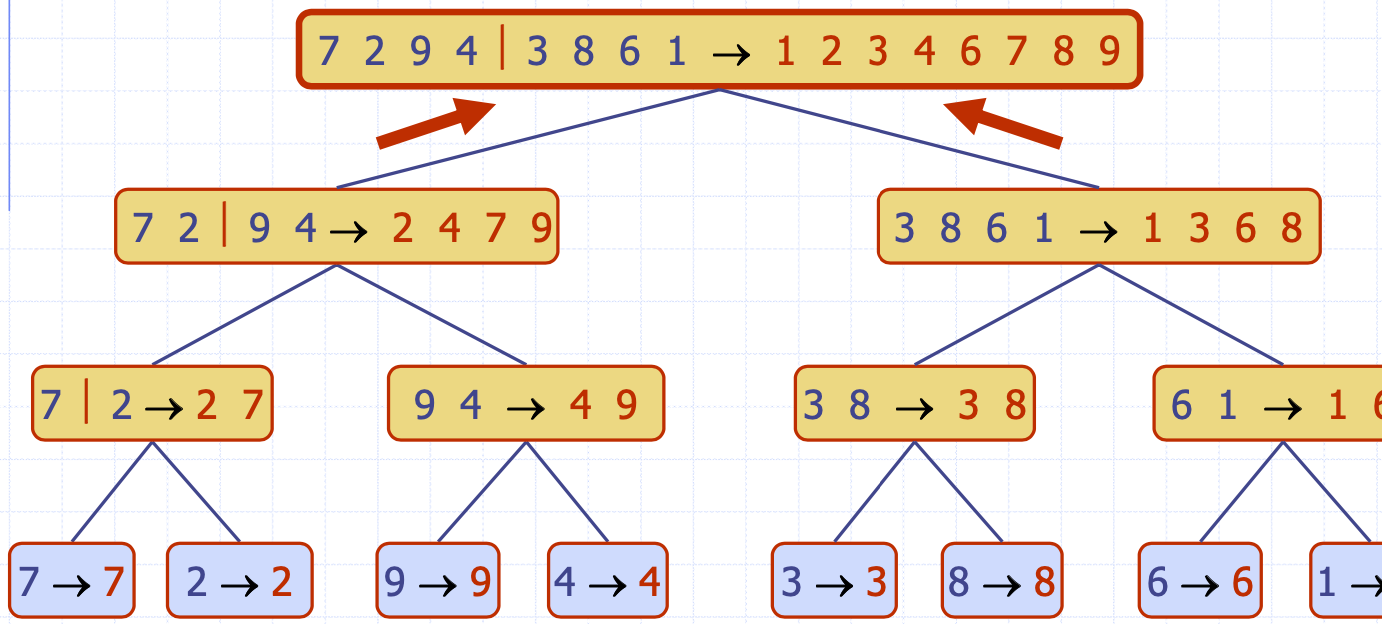
\includegraphics[scale=.2]{graphic/04 MergeSort/merge sort.png}
\end{center}


\paragraph{Laufzeiten}
\begin{center}
    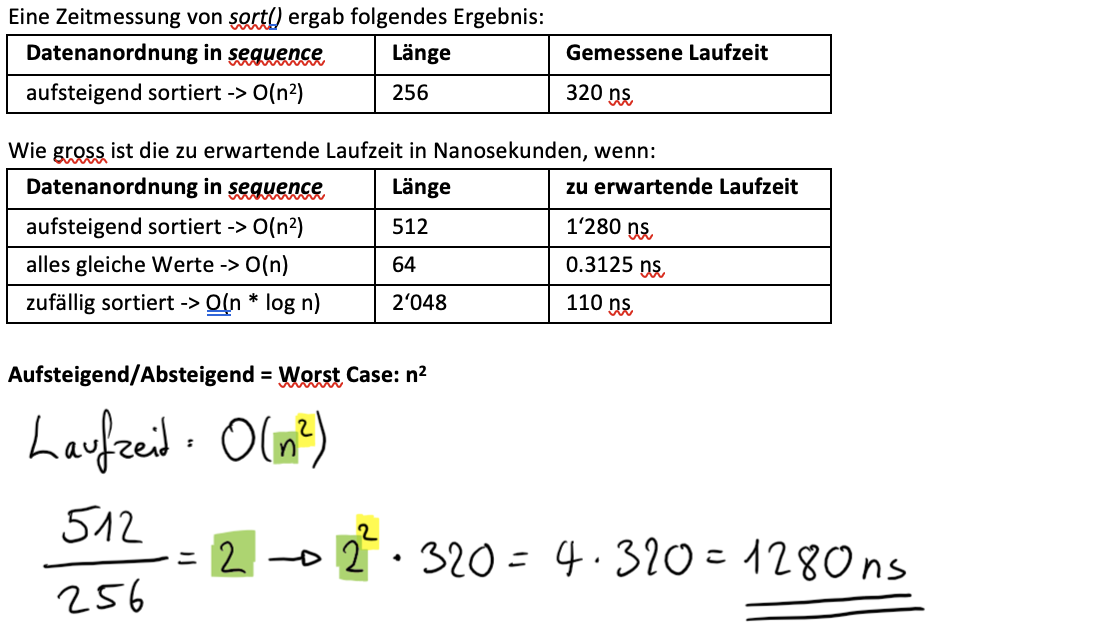
\includegraphics[width=\linewidth]{04 MergeSort/1.png}
    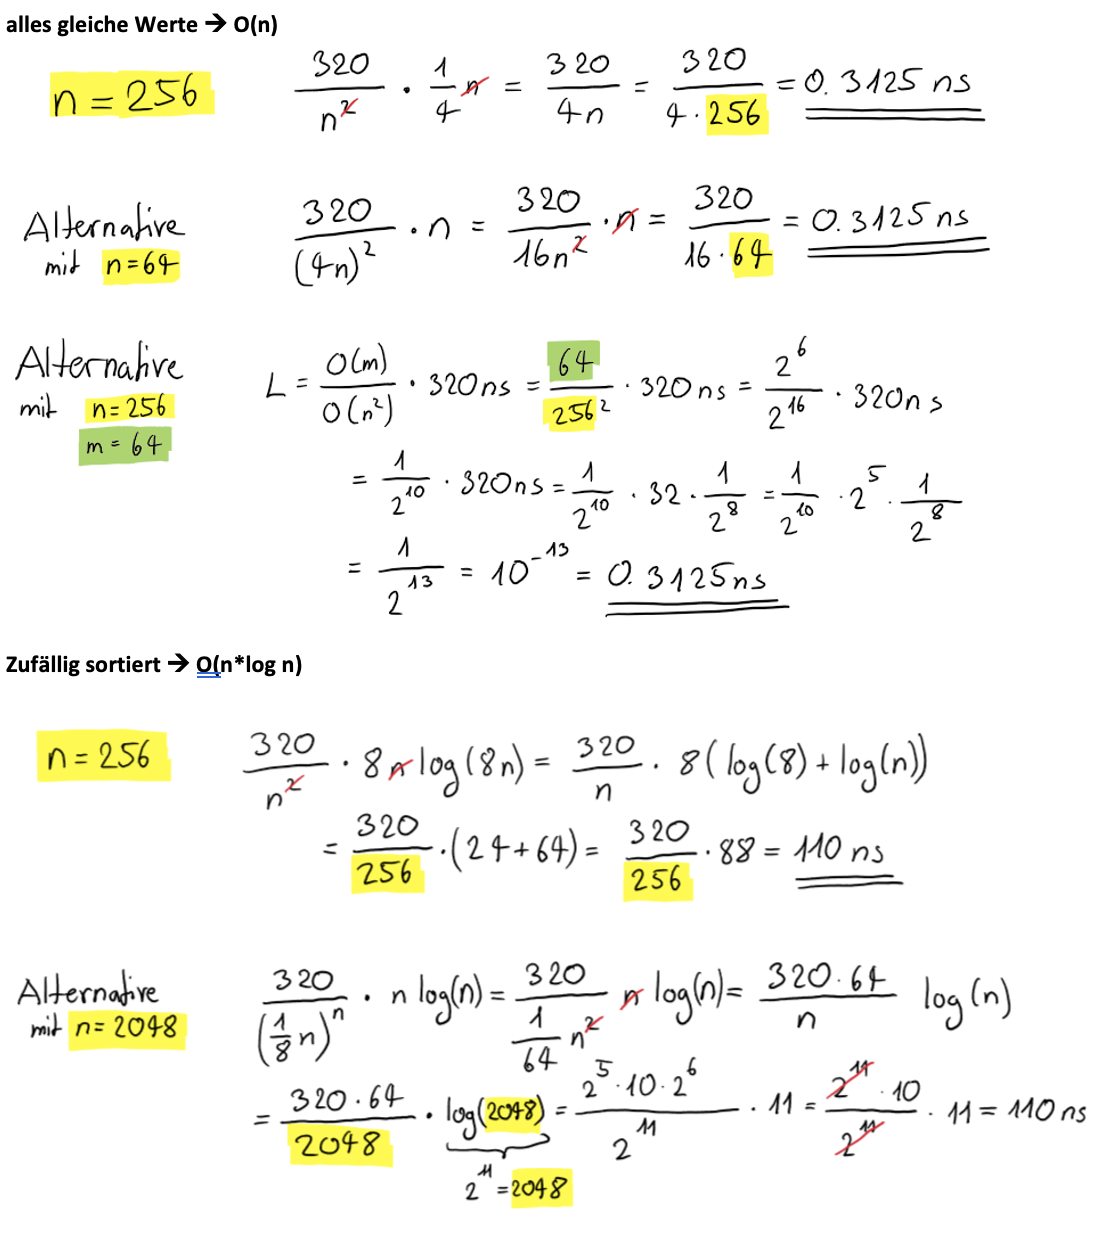
\includegraphics[width=\linewidth]{04 MergeSort/2.png}
    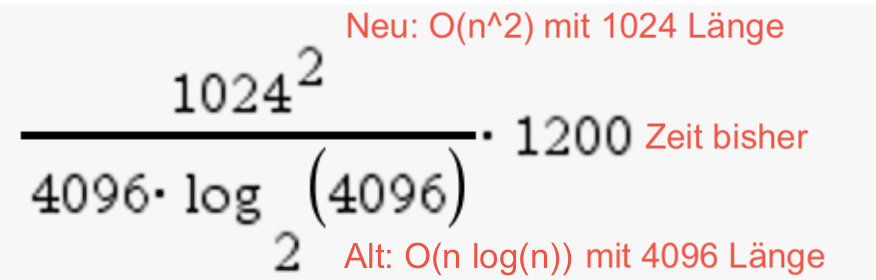
\includegraphics[width=\linewidth]{04 MergeSort/3.png}
\end{center}



\vfill


\paragraph{2-er Potenzen}
\begin{center}
    \begin{tabular}[]{| c | r || r | r |}
        \hline
        Potenz&Dezimal&Log&Dezimal\\
        \hline\hline
                    &           &   $log_2(0)$      & undef\\
        $2^0$       & 1         &   $log_2(1)$      & 0\\
        $2^1$       & 2         &   $log_2(2)$      & 1\\
        $2^2$       & 4         &   $log_2(4)$      & 2\\
        $2^3$       & 8         &   $log_2(8)$      & 3\\
        $2^4$       & 16        &   $log_2(16)$     & 4\\
        $2^5$       & 32        &   $log_2(32)$     & 5\\
        $2^6$       & 64        &   $log_2(64)$     & 6\\
        $2^7$       & 128       &   $log_2(128)$    & 7\\
        $2^8$       & 256       &   $log_2(256)$    & 8\\
        $2^9$       & 512       &   $log_2(512)$    & 9\\
        $2^{10}$    & 1'024     &   $log_2(1'024)$  & 10\\
        $2^{11}$    & 2'048     &   $log_2(2'048)$  & 11\\
        $2^{12}$    & 4'096     &   $log_2(4'096)$  & 12\\
        $2^{13}$    & 8'192     &   $log_2(8'192)$  & 13\\
        $2^{14}$    & 16'384    &   $log_2(16'384)$ & 14\\
        \hline
    \end{tabular}
\end{center}

